\chapter{Optimization derivations}
\label{app:gradients}
Using equations \ref{eq:cost} and \ref{eq:loss}, the goal is:
\begin{align*}
    \quad & \min_{\alpha, \beta} \mathbb{E} [\text{cost}(x, \alpha)] + \lambda \cdot \mathbb{E}[\text{loss}(x, \alpha, \beta)] \\
    &= \min_{\alpha, \beta} \mathbb{E} [\text{cost}(x, \alpha) + \lambda \cdot \text{loss}(x, \alpha, \beta)] \\
    &= \min_{\alpha, \beta} \frac{1}{D} \sum_{x \in D}[\text{cost}(x, \alpha) + \lambda \cdot \text{loss}(x, \alpha, \beta)].
\end{align*}
Here $D$ is the set of all target sentences. \\

\noindent Then $f$ can be defined as:
\begin{align*}
    f(x, z, \beta) = \text{length}(z) + \lambda \cdot (-\log p_{\beta}(x|z)).
\end{align*}

\noindent And $F$ as:
\begin{align*}
    F(x, z, \alpha, \beta) &= \mathbb{E}_{q_{\alpha}(z|x)} [[\text{length}(z) + \lambda \cdot (-\log p_{\beta}(x|z))]] \\
    &=^{\ast} \sum_{z\in Z} [q_{\alpha}(z|x) f(x, z, \beta)] \\
    &= \mathbb{E}_{q_{\alpha}(z|x)}[f(x, z, \beta)],
\end{align*}
where $Z$ consists of all the possible masks of size $x$.
In the step marked with *, the law of the unconscious statistician is used: $\mathbb{E}_{P(A)}[f(A)] = \sum_{a \in A}P(a)f(a)$. \\

\noindent Thus, the goal then becomes:
\begin{align*}
    \min_{\alpha, \beta} F(x, z, \alpha, \beta).
\end{align*}

\noindent The gradient with respect to $\alpha$ can be calculated as following:
\begin{align*}
    \nabla_{\alpha} F(x, z, \alpha, \beta) &= \nabla_{\alpha} \mathbb{E}_{q_{\alpha}(z|x)} [f(x, z, \beta)] \\
    &= \nabla_{\alpha} \sum_z [q_{\alpha}(z|x) f(x, z, \beta)] \\
    &= \sum_z \nabla_{\alpha} (q_{\alpha}(z|x) f(x, z, \beta)) \\
    &=^\ast \sum_z (q_{\alpha}(z|x) [\nabla_{\alpha} \log q_{\alpha}(z|x) f(x, z, \beta)]) \\
    &= \mathbb{E}_{q_{\alpha}(z|x)} [\nabla_{\alpha} \log q_{\alpha}(z|x) f(x, z, \beta)].
\end{align*}
In the step marked with *, a log-derivative trick is used: $\nabla_t \log h(t) = \frac{\nabla_t h(t)}{h(t)}$. \\

\noindent And the gradient with respect to $\beta$:
\begin{align*}
    \nabla_{\beta} F(x, z, \alpha, \beta) &= \nabla_{\beta} \mathbb{E}_{q_{\alpha}(z|x)}[f(x, z, \beta)] \\
    &= \nabla_{\beta} \sum_z [q_{\alpha}(z|x)f(x, z, \beta)] \\
    &= \sum_z \nabla_{\beta} (q_{\alpha}(z|x)f(x, z, \beta)) \\
    &= \sum_z (q_{\alpha}(z|x) [\nabla_{\beta} f(x, z, \beta)]) \\
    &= \mathbb{E}_{q_{\alpha}(z|x)} [\nabla_{\beta} f(x, z, \beta)].
\end{align*}


\chapter{Figures for results section}
\label{app:results}

\begin{figure}
    \centering
    \begin{subfigure}[b]{0.47\textwidth}
        \centering
        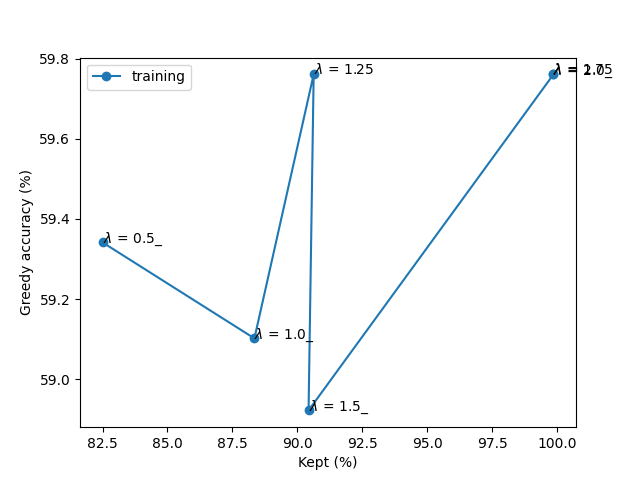
\includegraphics[width=1.1\textwidth]{figs/unstructured_acc_cost_train.png}
        \caption{Unstructured model, training set}
        \label{fig:unstr_train}
    \end{subfigure}
    \hfill
    \begin{subfigure}[b]{0.47\textwidth}
        \centering
        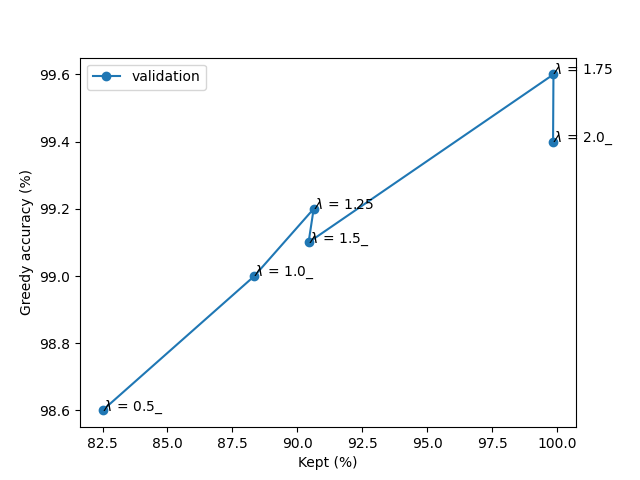
\includegraphics[width=1.1\textwidth]{figs/unstructured_acc_cost_val.png}
        \caption{Unstructured model, validation set}
        \label{fig:unstr_val}
    \end{subfigure}
    \hfill
    \begin{subfigure}[b]{0.47\textwidth}
        \centering
        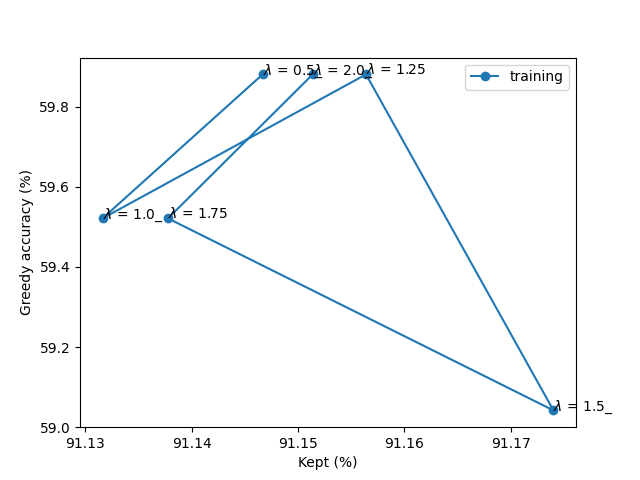
\includegraphics[width=1.1\textwidth]{figs/structured_acc_cost_train.png}
        \caption{Segmentation model, training set}
        \label{fig:str_train}
    \end{subfigure}
    \hfill
    \begin{subfigure}[b]{0.47\textwidth}
        \centering
        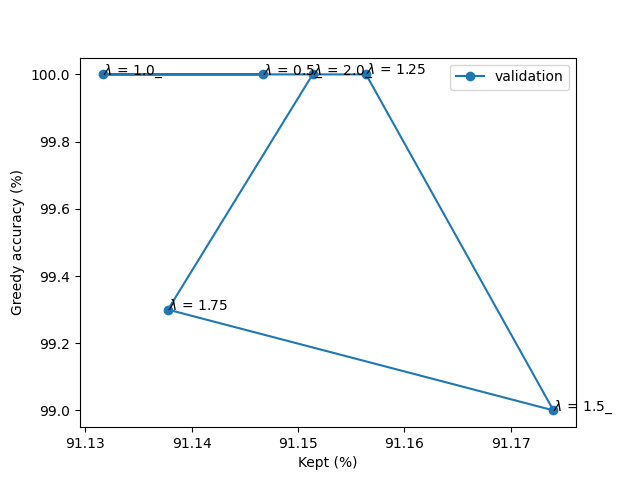
\includegraphics[width=1.1\textwidth]{figs/structured_acc_cost_val.png}
        \caption{Segmentation model, validation set}
        \label{fig:str_val}
    \end{subfigure}
    \caption{Accuracy and cost}
    \label{fig:acc_cost}
\end{figure}

\begin{figure}
    \centering
    \begin{subfigure}[b]{0.47\textwidth}
        \centering
        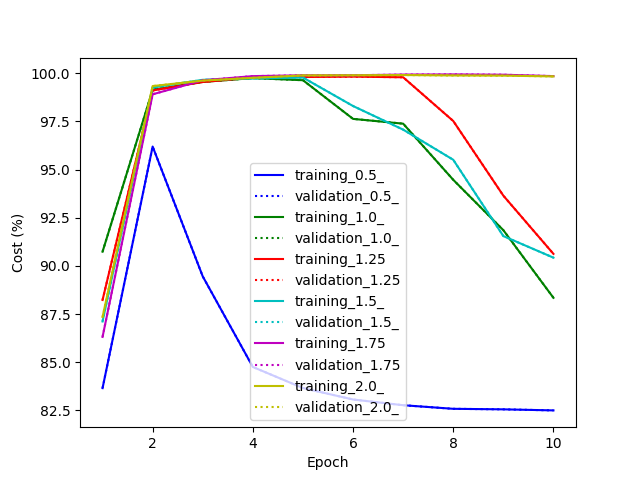
\includegraphics[width=1.1\textwidth]{figs/unstructured_cost.png}
        \caption{Unstructured model}
        \label{fig:unstr_cost}
    \end{subfigure}
    \hfill
    \begin{subfigure}[b]{0.47\textwidth}
        \centering
        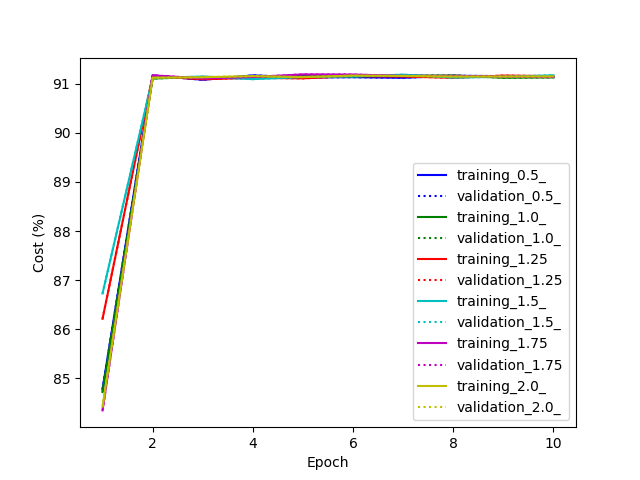
\includegraphics[width=1.1\textwidth]{figs/structured_cost.png}
        \caption{Structured model}
        \label{fig:str_cost}
    \end{subfigure}
    \caption{Cost}
    \label{fig:cost}
\end{figure}

\begin{figure}
    \centering
    \begin{subfigure}[b]{0.47\textwidth}
        \centering
        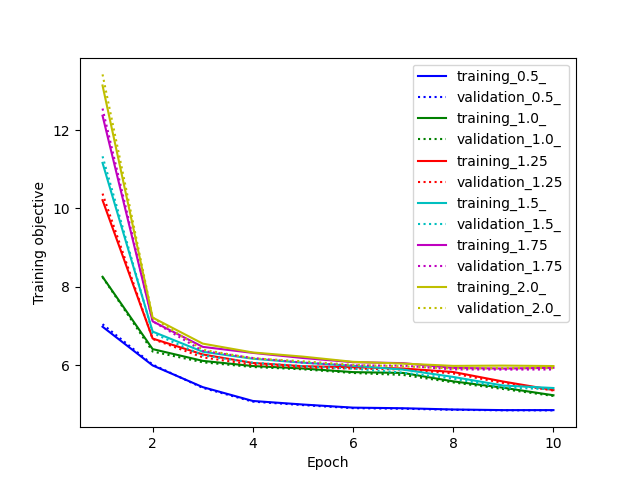
\includegraphics[width=1.1\textwidth]{figs/unstructured_obj.png}
        \caption{Unstructured model}
        \label{fig:unstr_obj}
    \end{subfigure}
    \hfill
    \begin{subfigure}[b]{0.47\textwidth}
        \centering
        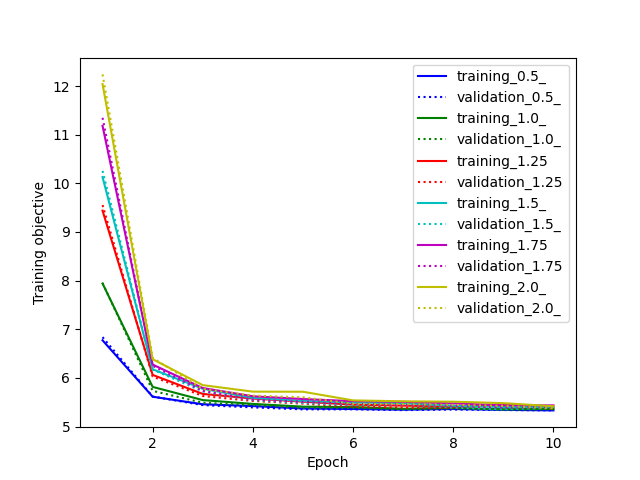
\includegraphics[width=1.1\textwidth]{figs/structured_obj.png}
        \caption{Structured model}
        \label{fig:str_obj}
    \end{subfigure}
    \caption{Training objective}
    \label{fig:obj}
\end{figure}

\begin{figure}
    \centering
    \begin{subfigure}[b]{0.47\textwidth}
        \centering
        \includegraphics[width=1.1\textwidth]{figs/high_acc_cost_val.png}
        \caption{Accuracy and cost}
        \label{fig:high_cost_acc}
    \end{subfigure}
    \hfill
    \begin{subfigure}[b]{0.47\textwidth}
        \centering
        \includegraphics[width=1.1\textwidth]{figs/high_cost_10000.png}
        \caption{Cost}
        \label{fig:high_cost}
    \end{subfigure}
    \hfill
    \begin{subfigure}[b]{0.47\textwidth}
        \centering
        \includegraphics[width=1.1\textwidth]{figs/high_obj_10000.png}
        \caption{Training objective}
        \label{fig:high_obj}
    \end{subfigure}
    \caption{Results with $\lambda = 10000$}
    \label{fig:high}
\end{figure}